\documentclass[a4paper, UTF8]{ctexart}
\usepackage[top=1.5cm,bottom=1.5cm,left=2cm,right=2cm,marginparwidth=1.75cm]{geometry}
\linespread{1.2}
\usepackage{amsmath}
\usepackage{tikz}
\usepackage{graphicx}
\usepackage{float}
\usepackage{listings}
\usepackage{caption}
\usepackage{fancyhdr}

\fancyhead{} % 删除所有页眉
\begin{document}
\pagestyle{plain}
\captionsetup[figure]{labelformat={default},labelsep=period}

\begin{figure}[H]
	\centering
	% \begin{framed}
	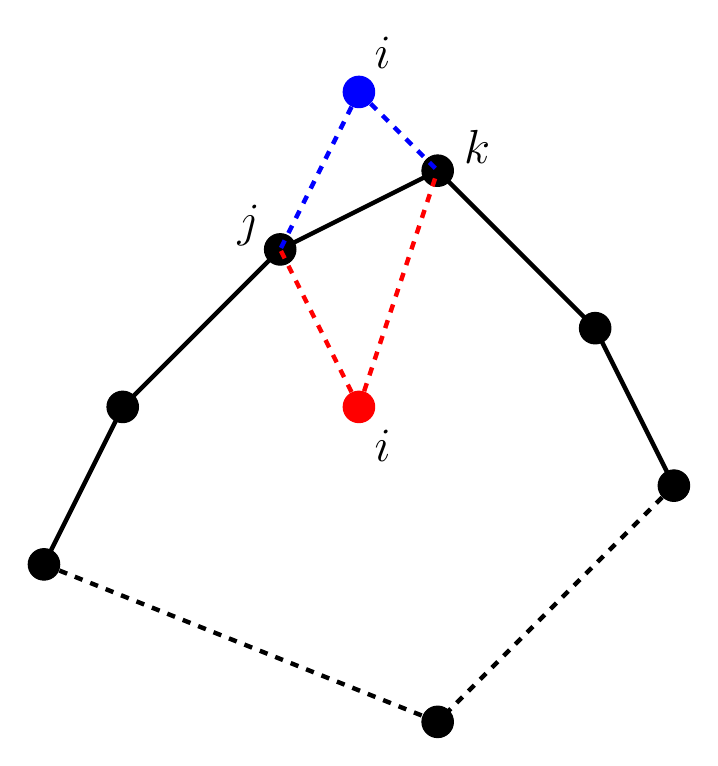
\begin{tikzpicture}

	\filldraw
		(0,0) circle (.2)
		(1,2) circle (.2)
		(3,4) circle (.2)
		(5,5) circle (.2)
		(7,3) circle (.2)
		(8,1) circle (.2)
		(5,-2) circle (.2)
	;
	\draw[ultra thick] (0,0)--(1,2) (1,2)--(3,4) (3,4)--(5,5) (5,5)--(7,3) (7,3)--(8,1);
	\draw[dashed, ultra thick] (0,0)--(5,-2) (8,1)--(5,-2);
	\filldraw[color=red] (4,2) circle (.2);
	\filldraw[color=blue] (4,6) circle (.2);
	\draw[dashed, ultra thick, color=red] (4,2)--(3,4) (4,2)--(5,5);
	\draw[dashed, ultra thick, color=blue] (4,6)--(3,4) (4,6)--(5,5);
	\node (i_1) at (4.3,1.5) [font=\fontsize{17.28}{0}\selectfont] {$i$};
	\node (i_2) at (4.3,6.5) [font=\fontsize{17.28}{0}\selectfont] {$i$};
	\node (j) at (2.6,4.3) [font=\fontsize{17.28}{0}\selectfont] {$j$};
	\node (k) at (5.5,5.3) [font=\fontsize{17.28}{0}\selectfont] {$k$};
	\end{tikzpicture}
	% \end{framed}
	% \caption{}
	\label{fig:1}
\end{figure}

\end{document}
